% Lösung bzgl. Zielsetzung -- Bezug zu methodischem Teil herstellen

% (Ist-Analyse)
\chapter{State of the art}
	
	% immer erwähnen, was man nutzt, und nie nur das
	
	This chapter examines noteworthy compiler generators as well as virtual machines
	%TODO and programming languages
	that influenced the design of the Perseus
	%TODO language and
	VM.
	
	\section{Common Compiler Generators}
    	
		Lexers and parsers are rarely hand-written any more, since there are plenty of tools to generate them using formal definitions. Let's compare some free and open source examples that can target C/{\CC} representing different approaches.
		
		First of all there's flex\cite{flex}, a classic lexer generator that creates C code from a definition file describing the tokens using regular expressions and code to be executed upon their recognition, for example suspending scanning and returning a token. The generated C source code is then compiled to get an executable lexer. flex is often used together with bison.
		
		bison\cite{bison} generates various kinds of LR parsers in C, {\CC} and Java from a definition file describing the context-free grammar to be accepted. The generated source code is then compiled to get an executable parser.
		
		Boost.Spirit\cite{spirit} is a {\CC} parser and lexer library. (It also has a module for generator definitions, but that is of no interest here.) It's different from flex and bison (and most other compiler generators) in that it doesn't have a separate generation step; the definitions are made in standard {\CC}.
		
		Boost.Spirit.Lex, its lexer component, lets you define the tokens using strings containing regular expressions. These are parsed and used to generate a deterministic finite automaton at run time, which has the downside that the computations will be repeated at each execution and syntactic errors in the regular expressions can't be detected during compilation. To offset this there's the option to generate equivalent static {\CC} source code for the calculated automaton on execution, which can then be used in place of the run time version for improved performance. Besides requiring no external tools for compilation it's also very easy to integrate with Boost.Spirit.Qi.
		
		Boost.Spirit.Qi is the parser component. Making heavy use of templates it allows for the definition of a parsing expression grammar using overloaded operators, creating a recursive descent parser. It eschews the packrat algorithm in favor of simple backtracking.

	\section{Common Virtual Machines}
		% Stand der Technik, insb. bzgl. VMs / Einordnung
		
		There are numerous virtual machines a compiler may target. One common example is the Java Virtual Machine (JVM), which was initially created for Java, but has since been targeted by other languages as well. It is stack-based and uses garbage collection to manage its memory.
		
		Another example, the LLVM is not just a virtual machine. It defines an Intermediate Representation for program code that compilers can target, much like byte code. It is then capable of optimizing it, compiling it to various machine code formats or executing it using on-demand compilation (JIT/Just In Time). It is register-based and supports both manual memory management and garbage collection, but no coroutines.
	
	%TODO \section{Selected Programming Languages}

% Anforderungsanalyse / Requirements
\chapter{Requirements}\label{requirements}

	%TODO where does this go? requirements? 
	%Native machine code would require porting work for each new platform. By using a virtual machine, any platform that's capable of running it is supported. My virtual machine requirements are mainly support for coroutines and stack inspection/unwinding, so coroutines can be serialized and aborted properly, and the ability to embed it in C++.
	
	This chapter lays down the precise requirements for the compiler and the VM\footnote{Those are the initial requirements for a first version, which can later be expanded; but that's outside of the scope of this thesis.}. Notably this includes the initial features of Perseus, the language to be compiled. It also explains why existing VMs don't fulfill these requirements, motivating the creation of a custom VM.

    \section{Target Language}
    
    	Eventually Perseus will be used as an embedded language, supplied as a library with functions to compile Perseus source code and execute functions in it. Initially that doesn't matter as much, just having some environment to execute Perseus scripts in is currently sufficient.
    	
    	The syntax should generally be based on Rust\cite{rust}, though only roughly; differences are acceptable. With that in mind, the following is what the language should be capable of initially.
    	
    	\subsection{Initial Feature-Set}
    	
			A Perseus program is made up of function definitions, one of which is called \lstinline$main()$ and is the entry point, for the time being. It has no parameters, but generally functions can have them and may be overloaded on them. The number and types of parameters are fixed, and functions are annotated with whether they are pure, i.e. side-effect free. Pure functions may only call other pure functions.
			
			Perseus scripts can also call native functions which have previously been registered. As a proof of concept an impure \lstinline$print(value)$ function will suffice initially; as the name suggests, it writes its single parameter to the standard output.
			
			To document Perseus scripts single- and multiline comments can be used. Multiline comments need not support nesting.
			
			The types initially supported are \lstinline$i32$, a 32 bit signed integer type, and \lstinline$bool$, a boolean type stored as a character since that is the smallest addressable unit. There's also a void type, \lstinline$()$, for statements. Arrays and record types are not initially supported, but will be added at a later time.
	    	
	    	The simplest expressions are literals: Constant values written directly in the code. Integer literals can be written in decimal (default), hexadecimal (prefix \lstinline$0x$) or binary (prefix \lstinline$0b$), with the option of using \lstinline$'$ as a separator, as in \lstinline$1'000'000$ or \lstinline$0b0010'1010$. Boolean literals are \lstinline$true$ and \lstinline$false$.
	    	
	    	Expressions can be combined using operators. In the future users will be able to define their own operators, including their associativity and precedence, so those should not be defined through the grammar but resolved at a later time. The predefined operators are given in table \ref{tab:perseus_operators}. Operators of same precedence with no associativity need explicit parentheses -- e.g. \lstinline$a==b==c$ is illegal.
	    	
	    	\begin{table}
			\begin{center}
			\begin{tabular}{ l l l l l }
			\toprule
			Symbol & Operands & Associativity & Precedence & Name \\
			\midrule
			\lstinline$*$ & \lstinline$i32, i32$ & left & 7 & integer multiplication \\
			\lstinline$/$ & \lstinline$i32, i32$ & left & 7 & integer division \\
			\lstinline$%$ & \lstinline$i32, i32$ & left & 7 & integer modulo \\
			\lstinline$+$ & \lstinline$i32, i32$ & left & 6 & integer addition \\
			\lstinline$-$ & \lstinline$i32, i32$ & left & 6 & integer subtraction \\
			
			\lstinline$==$ & \lstinline$i32, i32$ & none & 4 & integer equality \\
			\lstinline$!=$ & \lstinline$i32, i32$ & none & 4 & integer inequality \\
			\lstinline$<$  & \lstinline$i32, i32$ & none & 4 & less than \\
			\lstinline$<=$ & \lstinline$i32, i32$ & none & 4 & less than or equals \\
			\lstinline$>$  & \lstinline$i32, i32$ & none & 4 & greater than \\
			\lstinline$>=$ & \lstinline$i32, i32$ & none & 4 & greater than or equals \\
			
			\lstinline$==$ & \lstinline$bool, bool$ & none  & 4 & boolean equality \\
			\lstinline$!=$ & \lstinline$bool, bool$ & none  & 4 & boolean inequality \\
			\lstinline$&&$ & \lstinline$bool, bool$ & right & 3 & boolean and \\
			\lstinline$||$ & \lstinline$bool, bool$ & right & 2 & boolean or \\
			
			\lstinline$-$ & \lstinline$i32$  & & & integer negation \\
			\lstinline$!$ & \lstinline$bool$ & & & boolean negation \\
			\bottomrule
			\end{tabular}
			\caption{Predefined operators}\label{tab:perseus_operators}
			\end{center}
			\end{table}
			
			In the absence of error handling divide by zero currently leads to termination of the execution. For simplicity's sake there is initially no short-circuit evaluation for \lstinline$&&$ and \lstinline$||$\footnote{The absence of short-circuit evaluation means both operands are always evaluated, even if evaluating the left one suffices to determine the result.}; this may change in the future.
			
			``Block'' expressions contain multiple expressions to be executed serially; they may include variable definitions, which must include the initial value; its type can optionally be deduced from this. A variable is usable until the end of the block it was defined in. A block evaluates to the last expression in it.
			
			``If'' expressions evaluate to either their ``then'' expression or their ``else'' expression, depending on their condition, so both of those must have the same type. If the ``then'' expression is of type void, the ``else'' expression can be omitted.
        
        \subsection{Future features}
        	
        	Some future features should be kept in mind during implementation to ease their future addition. Besides the aforementioned user-defined types and operators, these are as follows:
        	
        	A UTF-32 string type. String literals will be UTF-8 encoded; scripts may therefore start with a UTF-8 Byte Order Mark\footnote{A special UTF-8 character signifying that the file in question is encoded in UTF-8.}.
        	
        	Coroutine support. %TODO say more here?
        	
        	Pointer types of some sort. Regardless of how exactly they look syntactically, there will at some point be a way to reference memory locations. This includes both the heap -- there will also be dynamic memory at some point -- and the stacks -- plural, since there's one for each coroutine.
        	
        	Serialization. There will be built-in support for serialization, with type annotations of some kind. Critically this will also include the ability to serialize paused coroutines (if the variables on their stack are serializable) so they can be resumed at a later date, possibly on a different computer. The use-case is a video game using Perseus scripts for its logic while allowing the player to save at any time, at which point a running script may need to be saved as well.
            
	
	\section{Compiler}
		
		The compiler is responsible for compiling Perseus scripts (as described above) into executable byte code for the VM. The input can be a file or a string from memory.
		
		It is important that the compiler tracks the current file location (at least the line, possibly also the column) so that error messages can include a location. It is acceptable for compilation to stop at the first error.
	
	\section{VM}
	
		The compiled byte code is run by a virtual machine so it can easily be executed on different machines.
		
		This VM needs to allow for manual memory management, since that will be added to Perseus in the future; it must not require garbage collection of dynamic memory.
		
		It also needs to support coroutines. While not part of this thesis they too will be added to the language at a later point, so the VM must not prohibit that.
		
		And lastly it must allow for stack inspection so coroutines can be serialized and safely aborted. Serialization will be one of the main features of Perseus in the future, so it's imperative that it can be implemented.
		
		\subsection{Suitability of existing VMs}
		
			The author of this thesis is not aware of any mainstream VMs that fulfill these requirements. The JVM and the Common Language Runtime\footnote{The VM targeted by C\#} are unsuitable because they force the use of garbage collection, while LLVM has no support for coroutines.

\chapter{Design} %TODO better name?
% Ansatz, d.h. z.B. Architektur, Module und ihre Kommunikation

	This chapter describes the design of the compiler and the VM: How were they supposed to fulfill the requirements?

	\section{Choice of implementation language}
	
		When it came to choosing a language to implement the compiler and VM in, there were multiple considerations.
		
		First of all the language should be widely available. Since Perseus will only ever run on a system supported by its host language, a mainstream language should be used.
		
		Perseus will at some point be usable as an embedded language, i.e. as a library. So it should be implemented in a language that can create widely usable libraries.
		
		And the language should make writing correct code easy while being powerful enough to write a useful compiler in it.
		
		With that in mind {\CC} was chosen. It is widely supported and compiles to native code; it supports and encourages the use of RAII to prevent resource leaks; and modern features introduced in {\CC}11 and {\CC}14 further simplify the writing of fast, correct code\cite{effective-modern-cpp}. It is also reasonably simple to write a C binding in it, and C libraries are widely supported.
		
		Since the author of this thesis primarily uses Windows for development, the compiler of choice was the release candidate of the Microsoft Visual {\CC} Compiler 2015. The previous 2013 version is severely lacking in {\CC}11 and {\CC}14 support, much of which was added for the 2015 version. But the final version of that was not yet released when development began, so it started on the release candidate, which was the latest available version at the time, although there was an upgrade to the final version after it was released later during development.
	
	\section{Choice of libraries}
	
		Parsers are not typically hand-written, since there are plenty of generators that create them based on a formal grammar. Out of them Boost.Spirit was chosen to implement the Perseus compiler. Boost.Spirit is a part of Boost, a widely-used set of {\CC} libraries covering many areas.
		
		There were multiple reasons for choosing Boost.Spirit: Firstly, the generator needed to work with {\CC}, the implementation language; all Boost libraries are strictly for {\CC}. Its use of Parsing Expression Grammars instead of LL or LR grammars simplifies the grammar definitions, thanks to being inherently unambiguous. And it doesn't require a separate generation step for the parser, relying instead on {\CC} templates resolved during normal compilation.
		
		An obvious alternative would have been using flex and bison; but having to define the language using an LR grammar would have added additional complexity and the additional build steps required to generate the source code based on the grammar/lexer definitions are undesirable.
		
		So since there was thus already a dependence on Boost, it was obvious to use Boost.Test for unit testing. Not only is Boost.Test capable of running a wide range of user-defined checks and reporting failures, it also detects memory leaks.
	
	%TODO Namespaces - perseus / perseus::detail (?)
	
	\section{Modules}
	
		% I suppose a diagram would be useful here?
		
		There are two distinct components: The compiler and the VM. The interface between the two is the byte code which the compiler generates and the VM executes.
		
		\subsection{Byte code}
			
			The byte code contains a sequence of instructions, which consist of an opcode and possibly one or more operands. Instructions thus vary in length, so the byte code is stored in a dynamic array of bytes; essentially raw memory, pieces of which are then interpreted as instructions. While this has the potential for misinterpretation when the piece of memory being interpreted is mid-instruction, a correct compiler will only ever create valid byte code that never jumps into the middle of an instruction.
			
			This has the advantage of being very compact; equally sized instructions would usually be much larger than necessary to accommodate for the largest ones. In an effort to further reduce byte code size, opcodes are of varying length as well. To this end they are encoded such that the number of consecutive 1-bits in the first byte indicates the number of additional bytes of the opcode\footnote{This is much like the UTF-8 encoding, but unlike there continuation bytes are not explicitly marked here.}. So if the most significant bit is 0, it's a single-byte opcode; there are 128 of those, due to the 7 remaining bits. For example \lstinline$0010'1010 = 42$ and \lstinline$1000'0101 0011'1001 = 1337$.
			
			Stack-based instructions are used instead of register-based ones because they're simpler; they implicitly operate on the values on top of the stack, making them well suited for evaluating expressions without the need for register allocation. They tend to require more copies to get the necessary values on top of the stack, but that's an acceptable price for simplicity.
			
			The essential initial instructions are integer arithmetic and boolean operations (one instruction for each of the operations defined in table \ref{tab:perseus_operators}), instructions for pushing integer and boolean constants, popping memory and copying values from and into the stack, as well as various types of jumps (including conditional jumps for branching) and call and return instructions.
			
			Generally the goal was to have a reduced instruction set: Only have a handful of simple instructions that can be combined to achieve more complicated tasks. This makes the VM simpler; and if the efficient execution of complex tasks is required, native function calls can be used.
			
			% [Note: I can't actually write about the calling convention, because on second thought I should have probably used a different one...]
			% Calls need a convention for their parameters and return values: How are they passed? A convention in keeping with the stack-based approach would be for the caller to push the parameters, then call the function; the function would then pop the parameters from the stack and leave the result in their place.
		
		\subsection{Compiler}
			
			The first steps of compilation are an ordinary lexer and parser. The following semantic analysis is done in two passes: First the function signatures are extracted to allow for forward references; in the second pass variable and function usages are resolved, types determined and the syntax tree is generally transformed as necessary. Finally code generation traverses this transformed syntax tree and writes the byte code.
			
		\subsection{Virtual Machine}
			
			At its core the VM has a simple fetch \& execute loop: Read the next instruction, act accordingly, repeat.
			
			What instruction is read depends on the location of the instruction pointer, which points into the code segment containing the byte code and is advanced whenever it is read from.
			
			Since multiple coroutines will be required in the future, they are already modeled in the VM, although there is only one at the moment. They are tracked by a coroutine manager. A coroutine has its own instruction pointer and stack; together those represent the current state of a coroutine and will be serializable in the future. There is no type information on the stack; in the future it will be precomputed for yielding functions, but since it will be required so infrequently it is not part of the stack.
			
			The size requirements of those stacks vary wildly: Complex coroutines might need a lot of stack to do large computations, but there can also be many simple coroutines which just need a little. In the interest of only using as much memory as necessary stacks are thus implemented as dynamic arrays. Since those may move in memory when they are reallocated with a larger size, a level of indirection will be required for stack pointers once those are added; but they are not yet required, since memory currently only needs to be accessed relative to the top of the current stack -- to access function parameters, local variables and set the return value.
			
			The instruction pointers point into the code segment, which encapsulates the byte code generated by the compiler.
			
			All these elements are modeled as classes. Their general relationships are shown in the class diagram in figure \ref{fig:vm_class_diagram}; it also shows the processor class which contains the fetch \& execute loop and that (directly or indirectly) has ownership of objects of the other classes.
			
			\begin{figure}
			\centering
			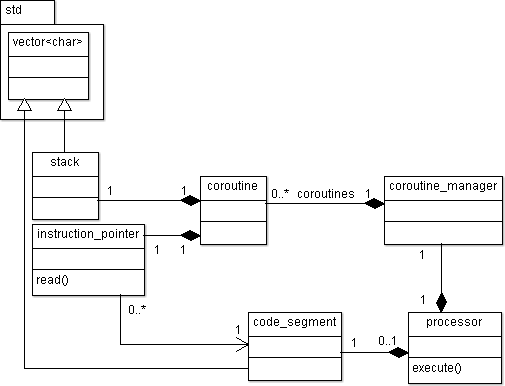
\includegraphics[width=\textwidth]{figures/vm_classes_cropped}
			\caption{VM class diagram (planned)}
			\label{fig:vm_class_diagram}
			\end{figure}

% Entwicklungsanalyse
\chapter{Implementation}

	% Umsetzung wesentlicher Module, ggf. Quellcode-Ebene
	This chapter selectively highlights the actual implementation: What difficulties came up? How are the libraries used? What interesting decisions were made?
	
	\section{Lexer \& parser}
		
		As mentioned Boost.Spirit was used to implement both the parser and the lexer. Figuring out how exactly to use it was slightly troublesome because its documentation is mediocre. While it contains most important information somewhere, it's often difficult to find the relevant pieces; and usually no lexer is used, the grammar is instead defined directly in terms of characters. Luckily there are various examples in addition to the documentation which show most features in action.
		
		Incorrect usage usually results in compile errors though, so it is at least obvious that there is a problem. While the errors tend to be heavy in templates and many lines long, making them hard to understand, Boost.Spirit makes an effort to help, providing comments with explanations at common error sources.
		
		%TODO Iterators
		
		\subsection{Lexer}
				
		For the lexer token names are defined using an enumeration, which is supplied to the lexer as a template parameter. Their regular expressions are then defined as shown in listing \ref{lst:impl_lexer}, with the order implying their precedence. So while ``let'' also matches the \lstinline$identifier$ pattern, the \lstinline$let_$ pattern is chosen because it is defined first.
		
		\cppinclude[caption={Token definitions in Boost.Spirit.Lex},label={lst:impl_lexer}]{listings/tokens.cpp}
		
		%TODO UTF-8/UTF-32? BOM at least?
		
		\subsection{Parser}
		
		Grammar definitions are more complex, since they may yield\footnote{Not yield in the coroutine sense; but these results are passed using reference parameters, so ``return'' is inappropriate.} nodes of the syntax tree. To this end the rules describing the non-terminal symbols have a template parameter defining the type to be yielded. Keywords for example carry no further information, as exemplified by the \lstinline$let$ keyword in listing \ref{lst:token}, while a constant yields a leaf node containing its value.
		
		\cppinclude[caption={Using tokens (terminal symbols) in the grammar},label={lst:token}]{listings/grammar_token.cpp}
		
		Leaf nodes are of limited use, nodes need to be combined to get useful syntax trees. The two most common operators to this end are the sequence and the alternative. Generally an alternative yields a \lstinline$boost::variant$ and a sequence yields a tuple. But these results are collapsed according to various rules\cite{spirit_attributes}; for example any symbol that yields no result is omitted, and if both alternatives yield the same type of result, there's no need for a \lstinline$variant$. It is also possible to define conversions from tuples to structs, making them much easier to handle.
		
		This is exemplified in listing \ref{lst:sequence_alternative}. \lstinline$attr( x )$ is a parser that consumes no input and yields its parameter \lstinline$x$; it is used in the \lstinline$optional_mutable$ rule to yield \lstinline$true$ in presence of a \lstinline$mutable_$ token and \lstinline$false$ otherwise. Since \lstinline$mutable_$ yields no result(see listing \ref{lst:token}), the result from the sequence of it and \lstinline$attr( true )$ is solely \lstinline$true$ -- if the parse is successful. Meanwhile \lstinline$deduced_variable_declaration$ is an example of a tuple being converted to a struct and \lstinline$block_member$ is an example for an alternative yielding a \lstinline$variant$.
		
		\cppinclude[caption={Combining non-terminal symbols in the grammar},label={lst:sequence_alternative}]{listings/grammar_sequence_alternative.cpp}
		
		Initially expressions were accidentally defined using left-recursion, i.e. one of its alternatives was akin to \lstinline$expression >> operator >> expression$. In the recursive descent parser this lead to infinite recursion, eventually causing a stack overflow. The chosen fix to this is outlined in listing \ref{lst:expression}; \lstinline$*$ is the Kleene star operator (used as a prefix due to {\CC} syntax), which yields a container (\lstinline$std::vector$ in this case) and one definition of \lstinline$operation$ is \lstinline$operator >> operand$. This results in a flat list of operations with no precedence resolution, which must not happen before the semantic analysis to support future user-defined operators with custom precedence.
		
		\cppinclude[caption={Defining expressions using operands and repetition},label={lst:expression}]{listings/grammar_expression.cpp}
		
		The whole grammar is described in this fashion. The result of parsing is a single syntax tree, which is then processed in the semantic analysis.
	
	\section{Semantic analysis}
		
		The semantic analysis visits the syntax tree, processing and transforming nodes. This is done under consideration of the context; what variables have been defined? Are there any restrictions on the type of variable allowed here? (``If'' conditions must be of type \lstinline$bool$, for example.) What functions are available? And so on. This information is therefore supplied in a context object, which can be adjusted as required.
		
		Of particular interest are \lstinline$boost::variant$ nodes, since they represent one of multiple possible types. They are processed using a visitor as outlined in listing \ref{lst:visitor}; types are distinguished through overloading of the call operator.
		
		\cppinclude[caption={Visitor for the \lstinline$boost::variant$ defined in listing \ref{lst:sequence_alternative}},label={lst:visitor}]{listings/visitor.cpp}
		
		These transforming functions return a different node type because the transformed syntax tree has different nodes; one example are operations: Initially they're in a flat list (see listing \ref{lst:expression}) but for proper code generation binary operations are required. This requires different nodes, which also have additional annotations like types.
		
		Types are still pretty simple. While eventually user-defined types will be introduced, for the moment there are only \lstinline$i32$, a 32 bit signed integer; \lstinline$bool$, a boolean type; and \lstinline$void$/\lstinline$()$. Those are simply implemented as an \lstinline$enum$.
		
		Semantic analysis also resolves variable references. To this end the context contains the current scope, i.e. the variables that have been declared, mapping their name to their type and position in the stack. When a variable is referenced, its name is looked up in the scope and its offset calculated and stored in its node in the syntax tree.
		
		\subsection{Function Manager}
			
			One interesting part of the semantic analysis is the function manager, which keeps track of all the function definitions. In this context operators are treated as functions, because they are: functions with two parameters (or one) that may be overloaded, like \lstinline$==$, which is defined for both integer and boolean values. Only the syntax for calling them is different from normal functions.
			
			In a first pass through the syntax tree all function definitions are collected and stored in the function manager; this allows for forward references. A second pass then does most of the transformations and checks.
			
			A function is identified by its signature, which is its name and the types of its parameters. This allows for overloading. The functions are therefore stored as \lstinline$std::map<function_signature, function_info>$: A map from signature to function info. Function info includes its return type, whether it's a pure function (i.e. free from side effects), its operator precedence and its address as well as a list of address requests.
			
			The address is the location of the function in the byte code: What address do you call to run this function? Since in the case of forward references a function is called before its code has been written (and thus its address determined), such calls use a placeholder while their address is stored in the request list. That way once the address is known all previous placeholders can be replaced.
			
			Functions are looked up based on their signature during the semantic analysis. The result is cached so no additional lookup is required during code generation; to this end the function call node is annotated with the function's entry. Entries in an \lstinline$std::map$ are usually referred to by an iterator, which is used much like a pointer but is capable of advancing to the next element of a container, which pointers can only do in arrays. In debug builds iterators often also perform various checks: It is illegal to use an iterator after the object it points into has been destroyed, for example, so a debug container might keep track of its iterators and invalidate them upon its destruction, causing them to fail blatantly in case of future use, instead of potentially undefined behavior.
			
			So naturally iterators were initially used to refer to entries in the function map. Surprisingly this lead to crashes at runtime; more surprisingly these were caused by the code checking for invalidated iterators, yet they were not due to those checks catching errors, the error appeared to be within the checks themselves. But a fix could not be found and time was running out, so as a last resort pointers were used in lieu of iterators. This was technically still valid code; it no longer had the presumably broken correctness checks, but it didn't crash any more and appeared to be working correctly.
			
			Later the compiler was updated; the final version of Visual Studio 2015 was released and replaced the previously used release candidate for development. Now the original iterator code worked again; apparently the issues were indeed caused by an error in the compiler.
		
	\section{Code Generation}
		
		After the transformations are done, the new annotated syntax tree is traversed and its byte code is generated. Once again the necessary context is kept in an object; this includes the current size of the function's stack so the appropriate amount can be popped when writing a return, or at the end of a block when local variables go out of scope.
		
		The addresses for function calls are written using the function manager, which keeps tracks of forward references and writes the appropriate placeholders, overwriting them later as previously explained. In addition to this, there are occasionally relative jumps to unknown offsets, for example when jumping to the ``else'' branch of an ``if'' expression. This is handled very similarly to forward references in function calls: A placeholder is written, its address stored and its value replaced once it's known, i.e. after the ``then'' branch has been generated in this example.
		
		The code segment that the byte code is written into is just a dynamically sized chunk of memory, based on \lstinline$std::vector<char>$. Generally values are copied byte-wise to append them to the code segment. In this case it must be guaranteed that this is valid for the given types; objects with a special copy constructor can't just be copied verbatim in this way, for example. To this end a static assertion is used, which does the necessary check during compilation and causes an error if necessary.
		
		Opcodes however are handled differently; as previously explained they get encoded to save space. To this end the function for appending values to the code segment is specialized for opcodes, using the encoding function in those cases. See listing \ref{lst:code_segment_push} for the code behind this.
		
		\cppinclude[caption={Writing arbitrary values to the end of the code segment},label={lst:code_segment_push}]{listings/code_segment_push.cpp}
		
		\subsection{Opcodes}
			
			Opcodes are defined in a big enumeration, which also includes their documentation; for each instruction the behavior is defined, in particular what values are read from the code segment in addition to the opcode and what is read from or written to the stack. An example is given in listing \ref{lst:opcode}. The documentation uses Doxygen syntax so that it can be extracted automatically.
			
			\cppinclude[caption={Opcode documentation},label={lst:opcode}]{listings/opcode.cpp}
	
	\section{Virtual machine}
		
		Once the code segment has been generated it can be executed by the VM. This happens inside a loop which fetches the next instruction and executes it. To this end it uses an instruction pointer, which points inside the code segment at the next instruction to be interpreted and can be moved to implement jumps and calls. There's also the stack which is used for calculations; it too is implemented as a dynamic array so it can grow as necessary while being cache-friendly. In the interest of being future-proof the stack and the instruction pointer are part of a coroutine object. 
		
		The loop's basic structure is shown in listing \ref{lst:vm}: An instruction is read from the instruction pointer -- reading from it works much like writing to the code segment, in that there's a general function for arbitrary trivially copyable types and a specialization for opcodes, which need to be decoded -- and handled according to a huge switch statement, which is probably optimized using a jump table by the compiler to execute very quickly.
		
		\cppinclude[caption={VM execution loop (excerpts)},label={lst:vm}]{listings/vm.cpp}
		
		%\subsection{Native functions}
		
		Native functions are implemented using the \lstinline$syscall$ opcode. It has as its parameter an index into an array of native functions; the appropriate one is called with the current stack as the parameter so it can access the parameters and write the result. The appropriate function entry is then manually added in the function manager and a small function containing the syscall written to the code segment. The native function is responsible for keeping the stack intact and writing its results to the right place; eventually there will be a type-safe wrapper for this.

%%%%%%%%%%%%%%%%%%%%%%%%%%%%%%%%%%%%%%%%%%%%%%%%%%%%%%%
% Schluss: Wichtigster Teil (zusammen mit Einführung) %
%%%%%%%%%%%%%%%%%%%%%%%%%%%%%%%%%%%%%%%%%%%%%%%%%%%%%%%

\chapter{Evaluating the results}
% Zusammenfassung
% What did I achieve?
% Ergebnisse zusammenfassen, bewerten bzgl. Zielsetzung, Perspektiven
% lessons learned
This chapter examines the resulting compiler and VM: Do they fulfill the requirements? What does a Perseus program look like and how does the compiler translate it into executable byte code?

The goal was mostly reached: A small core of Perseus can be compiled and executed. Compared to the desired target language example (Listing~\ref{lst:target_language}), this is what the actual syntax looks like:

\begin{perseuslisting}[caption={Actual resulting language example},label={lst:result_language}]
function fib( x : i32 ) -> i32
    if x <= 1
        x
    else
    	// precedence must be explicitly defined since function calls are syntactically treated similar to binary operators and operator precedence is not resolved yet.
        ( fib( x - 1 ) ) + ( fib( x - 2 ) )

impure function main()
{
	let index : i32 = 10;
	let result = fib( index );
	print( result )
}
\end{perseuslisting}

That's pretty much on target, sans operator precedence resolution. The error messages for invalid code still leave a lot to be desired though -- they often lack information on the location of the problem. It's technically possible to include this information, and it sometimes is included already, but it was no priority during initial development, so future work in this area is required.

Meanwhile the virtual machine already has support for coroutines in anticipation for their future addition to the language. New opcodes, e.g. for unsigned integer and floating point arithmetic, are easy to add. The main challenge in extending it will probably be the addition of stack inspection and unwinding.

One of the main difficulties during development was figuring out how exactly to use certain features of Boost.Spirit, the compiler generator used. It eventually did its job, removing an additional compiler generation step from the build process as intended; and by taking advantage of \CC's powerful static type system most errors could be caught at compile time.

Due to the usage of the latest {\CC}14 features on a preview release of the Microsoft Visual {\CC} Compiler, a couple of compiler bugs were encountered, but its usage was still justified in that it made writing fast, correct and elegant code noticeably easier than it would have been in {\CC}98. The compiler has since had its full release, which fixed all the bugs that had been encountered.


\section{Resulting translation by example}

Taking listing \ref{lst:result_language} as an example, what do the steps of compilation look like? First, the lexer turns the source code into the following token stream (whitespaces and comments are omitted in this listing for brevity, and some indentation was added to aid comprehension):

\begin{codelisting}[caption="Abridged tokens of listing \ref{lst:result_language}"]
"function", identifier(fib), "(", identifier(x), ":", identifier(i32), ")", "->", identifier(i32),
    "if", identifier(x), operator(<=), decimal literal(1),
        identifier(x),
    "else",
        "(", identifier(fib), "(", identifier(x), operator(-), decimal literal(1), ")", ")", operator(+), "(", identifier(fib), "(", identifier(x), operator(-), decimal literal(2), ")", ")"

"impure", "function", identifier(main), "(", ")",
"{"
    "let", identifier(index), ":", identifier(i32), "=", decimal literal(10), ";"
    "let", identifier(result), "=", identifier(fib), "(", identifier(index), ")", ";"
    identifier(print), "(", identifier(result), ")",
"}"
\end{codelisting}

The parser builds the syntax tree shown in figure \ref{fig:result_language_parser_tree} from these tokens. This syntax tree is then transformed in various ways: Expressions are rearranged, variable references resolved, types checked etc. The result is the transformed syntax tree shown in figure \ref{fig:result_language_transformed_tree}. Based on that byte code is generated -- listing \ref{lst:result_bytecode} shows the generated ``fib'' function in humanly readable format.

\begin{figure}
\centering
\begin{forest}
[\textit{file}
	[{fib() $\rightarrow$ i32}
		[\textit{arguments}
			[{x : i32}]
		]
		[\textit{expression}
			[\textit{operand}
				[\textit{if}
					% x <= 1
					[\textit{expression}
						[\textit{operand}
							[x]
						]
						[\textit{operations}
							[{$<=$}
								[{$1$}]
							]
						]
					]
					% x
					[\textit{expression}
						[\textit{operand}
							[x]
						]
					]
					% fib(x-1) + fib(x-2)
					[\textit{expression}
						[\textit{operand}
							% fib(x-1)
							[\textit{expression}
								[\textit{operand}
									[fib]
								]
								[\textit{operations}
									[\textit{call}
										[\textit{expression}
											[\textit{operand}
												[x]
											]
											[\textit{operations}
												[{$-$}
													[{$1$}]
												]
											]
										]
									]
								]
							]
						]
						[\textit{operations}
							[{$+$}
								% fib(x-2)
								[\textit{expression}
									[\textit{operand}
										[fib]
									]
									[\textit{operations}
										[\textit{call}
											[\textit{expression}
												[\textit{operand}
													[x]
												]
												[\textit{operations}
													[{$-$}
														[{$2$}]
													]
												]
											]
										]
									]
								]
							]
						]
					]
				]
			]
		]
	]
	[{main() $\rightarrow$ ()}
		[{[omitted for brevity]}]
	]
]
\end{forest}
\caption{Abridged syntax tree of listing \ref{lst:result_language}}
\label{fig:result_language_parser_tree}
\end{figure}

\begin{figure}
\centering
\begin{forest}
[\textit{file}
	[{fib() $\rightarrow$ i32}
		[\textit{expression}
			[\textit{if}
				[\textit{expression} : bool
					[{$<=$}
						[\textit{expression}
							[i32 var at -8]
						]
						[\textit{expression}
							[$1$]
						]
					]
				]
				[\textit{expression}
					[i32 var at -8]
				]
				[\textit{expression}
					[{$+$}
						[\textit{expression}
							[fib()
								[\textit{expression}
									[{$-$}
										[\textit{expression}
											[i32 var at -12]
										]
										[\textit{expression}
											[$1$]
										]
									]
								]
							]
						]
						[\textit{expression}
							[fib()
								[\textit{expression}
									[{$-$}
										[\textit{expression}
											[i32 var at -16]
										]
										[\textit{expression}
											[$2$]
										]
									]
								]
							]
						]
					]
				]
			]
		]
	]
	[{main() $\rightarrow$ ()}
		[{[omitted for brevity]}]
	]
]
\end{forest}
\caption{Abridged transformed syntax tree of listing \ref{lst:result_language}}
\label{fig:result_language_transformed_tree}
\end{figure}

\begin{codelisting}[caption="Byte code translation of function fib() in listing \ref{lst:result_language}",label={lst:result_bytecode}]
; this byte code for fib() starts at address 26
relative_load_stack size=4 offset=-8
push_32 value=1
less_than_or_equals_i32
; if
relative_jump_if_false offset=14
; then
	relative_load_stack size=4 offset=-8
	relative_jump offset=51
; else
	reserve size=4
	relative_load_stack size=4 offset=-12
	push_32 value=1
	subtract_i32
	call address=26 ; recursive call
	reserve size=4
	relative_load_stack size=4 offset=-16
	push_32 value=2
	subtract_i32
	call address=26 ; recursive call
	add_i32
relative_store_stack size=4 offset=-16
pop size=4
return parameter_size=4
\end{codelisting}

\chapter{Future prospects}
% Ausblick
%*  [Future plans/possibilities]
This chapter details possible future changes to the compiler and VM, explaining how the Perseus language might change.

As mentioned only a very simple core of the language has been implemented; there is a lot of room for improvement. There are a couple of comparatively simple features that can be added immediately, but few of them make the language any more powerful. Such changes are for the most part larger in nature, requiring more work, but they are required for the language to become viable.

    \section{Simple changes}
    
    	\subsection{Operator precedence resolution}
    	
    	The most important change at the moment is probably the resolution of operator precedence. Having to manually define precedence using parentheses is inconvenient at best and downright ridiculous in the case of function calls; having to write \lstinline$(myFunction()) + 1$ instead of \lstinline$myFunction() + 1$ is not acceptable in any way, although in that particular case changes to the grammar may a better solution.
		
		\subsection{Variable assignments}
		
		There is also currently no way of changing a variable's value; all variables are effectively immutable. To enable usage of iterative algorithms assignment is necessary, and adding it is fairly straightforward, since determining a variable's location in memory has already been solved for usage of variables in expressions.
		
		\subsection{Tail recursion}
		
		Optimizing tail recursion calls to simply jump back to the beginning of the function is mostly a matter of recognizing them, in which case slightly different code is generated. Not a major change.
		
		\subsection{Better errors}
		
		The syntax tree is not sufficiently annotated with file locations to always get useful errors, but it could and should be.
		
		\subsection{Cleaner API}
		
		The header files are not currently sufficiently separated into interface and implementation; it should be made clearer to the user what they are supposed to include by having those headers in a separate directory.
	
	\section{Complex changes}
		
		\subsection{Upgrade to Boost.Spirit 3}
		
		The compiler currently uses version 2 of Boost.Spirit, which was the latest stable version when development started. The next version has since been released, with potential improvements in compile time, speed and ease of use. An upgrade should be considered while the code base is still relatively small, before adding many new features, because the new version is incompatible with the current one due to changed syntax.
		
		\subsection{New language features}
		
		Perseus still lacks many features, which need to be added in the future. These include modules, so the code can be separated into smaller pieces; a proper type system that lets the user define custom types; some form of dynamic memory management, on which strings depend; first class functions with closures; coroutines; and the persistence that is so central to the language.
